\chapter{Introduction}
\label{cha:Introduction}
Captivating intro.
%PH: trengs ikke


%You'll notice at the start I am correcting some style errors in the way or writing so that you can lift your way of writing already at this stage. many are just typical errors of how to write such a report. I am not correcting English, just general style... 
\section{Background and Motivation}\label{cit}
\label{sec:BackgroundAndMotivation}
%where's the motivation? You need to spell it out. What is the issue you are addressing and why is it important. 
%opening couple of sentences important.... 
The following research is situated within the area of hybrid algorithms.
More specifically, the research proposes a genetic algorithm used for classification. It differs from other genetic algorithms in that the goal is not to evolve a single individual capable of solving the task, but rather a whole population of capable individuals proficient at different parts of the task. Together the individuals approximate a complete machine learning function capable of classification. 

%bioinspired techniques are not machine learning....those are symbolic systems and these are sub.symbolic systems

The area of hybrid algorithms used for classification has been explored earlier [soruce plz]. Though, the novel idea for this research combining two well known techniques within GAs; namely the Island Model genetic algortihm (IGA) and artificial immune systems (AIS). These concepts will be elaborated in section\ref{sec:BackgroundAndMotivation}. %%avoid such statements. It is obvious when you start writing about them. Just introduce briefly and reference section with more information. 
The suggested algorithm, uses AIS for data classification and attempts to exploit the properties of an island based structure. Properties such as inherent parallelism and an ability to solve and combine subproblems, to increase both the accuracy and the efficiency of the classification process. Research already conducted indicate that a genetic algorithm developing in an island structure may provide enhanced results given that the problem consist of either linearly separable data points or sufficiently complex in terms of number of relevant attributes present in the data set used (Source plz). 

%Immune systems are not GAs. I find this intro to them too long. You are going into them but not really. Better to be very brief and refer forward than a half and half. almost introducing but not quite. 

%The island model can have effective convergence but it isn't taking any GA and helping it to converge. It is a variation of a GA that has a property of effective convergence
Artificial immune systems are a type of algorithms commonly applied to both optimisation and machine learning problems. AIS gets its name from the biological inspiration drawn from the immune system, and most often more specifically the adaptive immune system. Here a population of protein molecules called antibodies are evolved to recognise and attach to invading organisms referred to as antigens. In an AIS classification algorithm an input case is labelled by one or more antibodies that, with the the greatest degree of certainty, are able to recognise the case as some class \cite{AIS:Timmis2004}. 


\section{Goals and Research Questions}
\label{sec:Goals and Research Questions}
%%stating the obvious.....since you are presenting your goal then you have defined it. Take out any such phrases that don't really contribute anything... 
An overall goal for the research as well as some research questions for achieving this goal has been defined. The goal is defined as the overall question we wish to answer in this thesis while the research questions aim to decompose said goal into achievable sub-parts.

This section states the goal statement and research question that will be investigated in this thesis. The goal is set to open a path for research into this area of hybrid algorithms for classification. 

\begin{description}
\item[Goal] {\it How can artificial immune systems be combined with the island model to create an accurate and efficient novel hybrid classification algorithm.}
\end{description}
% never write "hope". Also "sufficiently"...what does that mean? Think about any such substantive words and if used they always need to be put in some kind of context. 
%Hopefully..... nope not that one either :) 
% think how the reader will interpret such phrases.....considerable further research.... whose..... considerable.....why do you think that.... also why would one research project into one hybrid algorithm ie one example and towards one application ever have a chance to have such an impact..... write more modest...not by using words like hope.,...but phrases like opening a  path for research into this hybrid algorithm for classification, or something like that. 
\noindent
%again empty phrase. 
To elaborate further, the suggested algorithm aims to use two well known techniques from biological inspired artificial intelligence, namely AIS and IGA. It is the combination of these two large and normally separate computational fields that makes this a hybrid algorithm. The task of classification will be handle by the implementation of the AIS, while the IGA will ensure a wider exploration of the search within the solution space.

%%Additionally, we have chosen to handle the machine learning aspect of the project by using artificial immune systems, a biologically inspired technique already known to have achieved success when applied to classification problems.
%you need to prove such statements with citations
%while this...what is "this". Again watch such words that can be hard for the reader to follow
%while this is not anything new.....correct but negative....say it in a more positive tone.... opr just remove and tell the reader what you are going to do... 

The wanted enhancements include improvements in both efficiency and accuracy, which means the algorithm should provide results with both a faster classification process as well as attaining more accurate results when compared to other algorithms running the same number of iterations. In the event that such results are not achieved, an explanation of why not, should be given under for the given conditions.

%The enhancements we are looking for include improvements in both efficiency and accuracy, meaning that we want to find conditions in which we achieve both a faster classification process while also attaining more accurate results when compared to other algorithms running the same number of iterations. In the event that we are not able to show this we aim to explain why satisfactory results were not achieved under the given conditions. 
%this last part is good but of course will need adjusted when the results are in.... this is motivation......should rewrite this in the first section that leads you into defining the goal

% your missing the important part...how best to combine... 
Much of the work in enhancing the classification process and result relies on exploiting the inherent parallel nature of the island model and its ability to effectively solve and combine sub-problems. However, we also aim to apply other improvements, specifically to the artificial immune system model used, to better suit the specific problem being solved and improve the performance of said part of the algorithm by itself.

%you are trying to increase these features of classification but relative to what? 
% Are you missing a question or an element of these questions that refers to finding out what type of problems can a such hybrid algorithm be best suited to. When is it worth the extra resources. That brings in another point. What is the cost of these increases? 
\begin{description}
\item[Research question 1] {\it How can the island model combined with artificial immune systems be used to increase the accuracy of the classification?}
\end{description}

\begin{description}
\item[Research question 2] {\it How can the island model combined with artificial immune systems be used to increase the efficiency of the classification process?}
\end{description}

\noindent
As the research aim to improve both accuracy and efficiency it is natural to look at these as separate goals before attempting to combine them.
%there may be a trade-off here that is worth thinking about
This means that the experimental plan first will focus on conditions in which accuracy is improved, followed by the conditions for efficiency. This is also reflected in the experimental plan in chapter \ref{cha:ResearchAndResults}. The specific improvements and conditions for achieving the different sub-goals might to some degree overlap. These characteristics will likely be important for achieving an algorithm that combines improvements to both efficiency and accuracy.
%maybe but you may also need to run experiments to improve both as well....or do you have a plan as to how to characterise the experiments in a way that you can identify such characteristics? If so, then identifying such characteristics may be a key element that needs to be in your research questions. 

\section{Research Method}
\label{sec:researchMethod}
The research method applied is first and foremost an analytic process. As our research objective is something that requires the combination of two established techniques that has yet to be attempted, it is more beneficial to look at the different research done on each technique individually. Using this research we inspect the different components of the techniques, their behaviour and impact on the result. Finding the different properties of the components and looking at how they could potentially positively affect an algorithm combining the techniques, is what has guided our structured literature search for the initial part of the project. 

Furthermore, we want to use the information and theories gathered from the literature search to create a model of such an algorithm. When choosing what components make up the model we naturally give preference to those which more likely yield a positively influence on the result. However, as we are pressed for time some more complex components will only be applied if time allows it and will be left to further research if not.
%this is fine here just now but will obviously be replaced as the project progresses. 

Finally, experiments will be conducted on the proposed model. Here we build a functional prototype of the algorithm and create experimental plans aimed at answering our research questions. The experiments will look at the two goals, efficiency and accuracy, separately and test parameters and components to enhance these qualities. 



\section{Structured Literature Review Protocol}

The following research questions and research strategy has guided the structured literature search in finding relevant articles for this thesis. This includes questions that have guided the search, as well as inclusion criteria that must be fulfilled for the article to be included, as well as the quality criteria to assess the value given to the research.

%% You state that quality criteria are not required. Why not? You then state that articles that are of higher quality..... how do you know they are better quality if you have not directly or indirectly applied some form of quality criteria?

\subsection{Research Questions}
As the project description was not set at the start of the project, the guiding research questions for the literature review has changed somewhat throughout the course of the search. However, one question that has been an important factor during the whole project is: "How can biologically inspired methods be fully integrated with machine learning in a classification system?". This was inspired by the fact that we early on knew we wanted to angle the project towards machine learning, and we noticed that most hybrid systems we looked at employed a two step process where standard machine learning was first applied and then some bio-inspired optimisation method was applied in the pre- or post-stages of the algorithm. 

As the project has gotten more targeted the search has changed towards questions focused more on specific techniques like artificial immune systems, the island model and generally hybrid algorithms. After deciding how to focus our research the following questions guided out literature search.

\begin{itemize}
  \item How can classification in artificial immune systems be enhanced?
  \item Under what conditions does use of the island model positively affect convergence and result?
\end{itemize}

This lead to further research into antibody shapes and techniques like local feature selection for enhancing AIS classification and specific migration policies, island architectures and conditions where the island model improves accuracy and efficiency of the algorithm. 

%fine at this time but the above section is something you should go back to and refine as the project progresses.  It is a bit incomplete. The last section leads on to believe that there are further sub questions. 

%think a bit about how easy it is for the reader to grasp what you have actually done here. the problem is again just text. The lack of tables or diagrams etc makes it hard to read and it is never the most exciting read anyway. Think how to present this in a clear fashion for the reader. 
\subsection{Research Strategy}
In attempting to answer these research questions a few quality and inclusion criteria has to be defined, as well as search engines keywords used when searching. These factors have been summarised in table \ref{table:litterature-review}. If the article is from a journal, the journal should hold a respectable score according to international standards as well to ensure that the information is credible.   

 \begin{table}[h]
        \centering
        \begin{tabular}{|l|l|}
        \hline 
        Identifying & 
                \begin{minipage}[t]{0.9\textwidth}
                        \textbf{Keyword used when searching (comma separated):}
                        \begin{itemize}
                        \item Artificial immune system, island based genetic algorithm, machine learning, classification, feature selection, migration, antibody shapes, clonal selection. \\
                        \end{itemize}
                \end{minipage}\\ \hline
        Qualifying  &  \begin{minipage}[t]{0.9\textwidth}
                        \textbf{Inclusion Criteria}
                        \begin{itemize}
                        \item  Articles have to have IGA or AIS as their main research topic.
                        \item The articles have to appear relevant from only reading the conclusion and abstract.
                        \item The articles should include a further work section that elaborate on possible improvements \\
                        \end{itemize}
                \end{minipage}\\ \hline
        Evaluating &  \begin{minipage}[t]{0.9\textwidth}
                        \textbf{Quality Criteria}
                        \begin{itemize}
                        \item The algorithms or techniques being presented in the research are compared against other algorithms  known  to  be  proficient  in  the  field  of  research  the  article  belongs to.
                        \item The article also needs to provide sufficient background information to understand the relevant topics presented.
                        \item The research must clearly state its purpose and it must be evident that it actually contribute to the field. \\
                        \end{itemize}
                \end{minipage}\\ \hline
        Including & \begin{minipage}[t]{0.9\textwidth}
                Research published by respected sources found on sites like IEEEXplore, ScienceDirect, Google Scholar, etc...  \\
                        \end{minipage} \\ \hline
        \end{tabular}
        \caption{Article Selection Criteria}
        \label{table:litterature-review}
\end{table}
    
% 5 years is regarded as recent.....
Furthermore, in a field where things change fast more recent articles are preferred. Preferably as recent as 2013 or later. However, given the nature of our research questions looking into concepts like island models in combination with machine learning, which is not something that, to our knowledge, has been researched before, this is not a strict limit. Since the amount of relevant articles is not abundant in the combination of the research fields that we have chosen, most of them addressing only one or a few parts of our research topics, it is important to also look at older articles as long as the research is at least partially similar and relevant to our research. Additionally, as most concepts in this search are new to us, we will at the start of our research prefer articles that gives us a broader understanding of the individual research topics, before focusing more on combinations of techniques as we become more knowledgeable about the base concepts. 

%To find relevant articles search queries should include a combination of relevant search words like \textbf{artificial immune system}, \textbf{island based genetic algorithm}, \textbf{machine learning}, \textbf{classification}, \textbf{feature selection}, \textbf{migration}, \textbf{antibody shapes}, \textbf{clonal selection}, as well as any abbreviation of these.

%Furthermore, a few quality and inclusion criteria has been defined to ensure that more useful articles are given greater preference. Articles will have to, at the very least, have IGA or AIS as their main research topic, and greater relevancy are given to articles with more of the included search terms as topics in the research \textbf{(IC1)}. The articles will also have to appear relevant from only reading the conclusion and abstract to be included \textbf{(IC2)}. Additionally, the articles should include a further work section that elaborate on possible improvements \textbf{(IC3)}. 

%A few quality criteria has been developed as well to assess the literature being reviewed. One such criteria is that articles are of greater quality when the algorithms or techniques being presented in the research are compared against other algorithms known to be proficient in the field of research the article belongs to \textbf{(QC1)}. Furthermore, comparisons of efficiency and accuracy are preferred. The article also needs to provide sufficient background information to understand the topics presented \textbf{(QC2)}. Finally, the research must clearly state its purpose and it must be evident that it actually contribute to the field \textbf{(QC3)}.

\section{Process}

%super figure. Just watch that you still want it to be a professional description of the thought process and thus statements like we did not like this or the "we" in general should be taken out. 

\label{fig:process}
\begin{figure}[H]
    \centering
    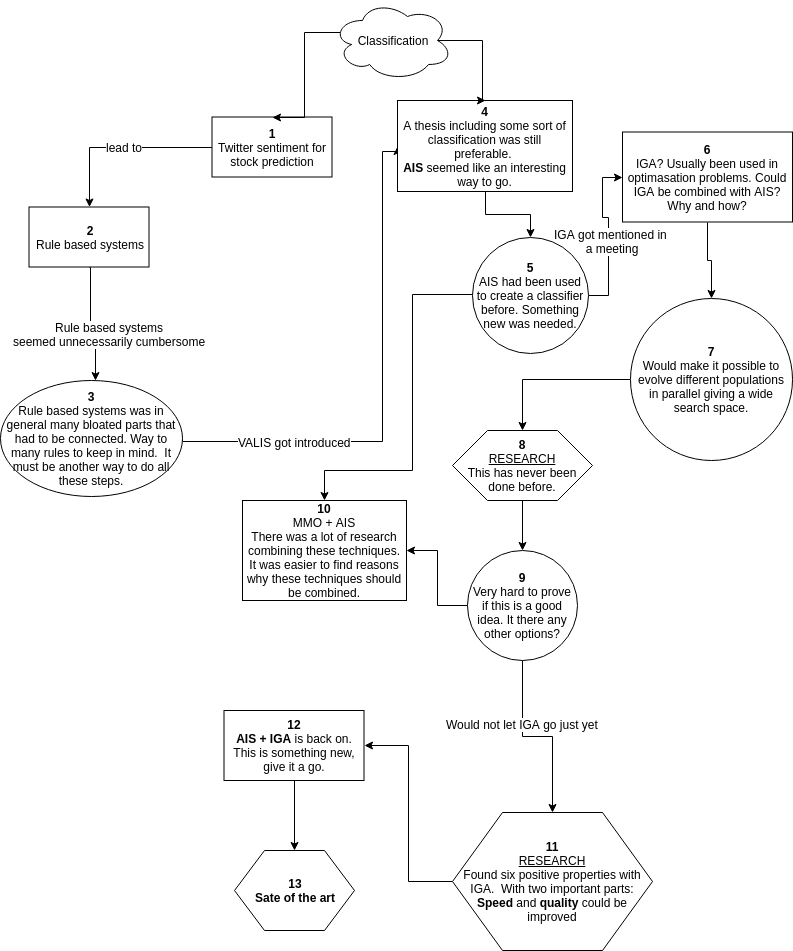
\includegraphics[width=0.9\columnwidth]{figs/process.png}
    \caption{Process overview}
    \label{fig:process_map}
\end{figure}

The creation of research a goal for this thesis were developed iteratively over time with research leading into several different fields, as shown in figure \ref{fig:process_map}. It started out with an article \cite{process:twitter-sentiment-ga} doing sentiment analysis on Twitter, optimised by a genetic algorithm to predict the stock market in the United States. The work of the article was focused heavily on the sentiment analysis and a support vector machine classifier and not on the genetic algorithm. It had a very complex and rule based model, which seemed unnecessarily complex. After a thorough literature review, the results showed that most research that combine machine learning and bio-inspired techniques are heavily module based.
%after a lot of research....whose? How does this module based result connect to the previous statement of unnecessarily complex. try to connect these sentences better. 
% missing some cites here to show a couple of examples that use such a module based approach
%"Proper"....not such a thing
One module would typically be a standard machine learning approach, while the steps of pre- or post-processing would be optimised with some sort of genetic algorithm. We concluded that it would be more interesting to fully integrate a genetic algorithm with machine learning to create a proper evolutionary machine learning algorithm, known as a hybrid algorithm. More research lead to the introduction of AIS through the VALIS algorithm \cite{process:valis}, which is an classification algorithm based on a vote allocating immune system. The possibilities with AIS was discussed, and it was found that in general AIS learning models encounter problems when working with higher-dimensional spaces \cite{AIS:representation-in-ais}.
%% there has been no discussion about geometric functions until now so the reader has no idea what this has to do with any AIS application here. even if this article states this you need to write in the context of your work here and use a cite that is appropriate. 
%%watch statements like "a lot of research was conducted"....it reads like we did a lot of work....try using things like a thorough literature review or something like that. ...or even just a review of the literature...... if you review, it takes time.... 
Therefore the idea of combining AIS with the island model was conceived. This topic was further researched, but we did not find any studies combining theses techniques. Subsequently, we concluded that the island model has mostly been used in optimisation problems, which made it difficult to find proof that combing it with AIS would improve the results of a classification algorithm. 

Since there was no evidence that a combination of AIS with IGA has even been attempted, it would be more sensible to look into other techniques for creating better classification algorithms. This lead to research done on multi-objective-optimisation (MOO), which had been combined with AIS already, making it easier to justify researching. However, the idea of combining AIS with the island model was more unique, which lead to another round of research with focus on the island model. This, in turn, lead to a list of positive properties with IGA techniques, where the two most important qualities was enhanced quality of the result and search speed. Finally, because of the promising articles found on our second research sequence into the IGA field, we decided to select our research objective as the creation a hybrid classification algorithm based on the IGA and AIS techniques. 

% once you lift the way of writing in the diagram and text then this will be a good section!


\section{Thesis Structure}
\label{sec:thesisStructure}

